\newcommand{\institut}{Institut f\"ur Energie und  Automatisiertungstechnik}
\newcommand{\fachgebiet}{Elektronische Mess- und Diagnosetechnik}
\newcommand{\veranstaltung}{Praktikum Messdatenverarbeitung}
\newcommand{\pdfautor}{\"Ozg\"u Dogan (326 048), Timo Lausen (325 411), Boris Henckell (325 779)}
\newcommand{\autor}{\"Ozg\"u Dogan (326 048)\\ Timo Lausen (325 411)\\ Boris Henckell (325 779)}
\newcommand{\pdftitle}{Praktikum Messdatenverarbeitung  Termin 7}
\newcommand{\prototitle}{Praktikum Messdatenverarbeitung \\ Termin 7}
\newcommand{\aufgabe}{}

\newcommand{\gruppe}{Gruppe: G1 Fr 08-10}
\newcommand{\betreuer}{Betreuer: J\"urgen Funk}

\input{../../packages/tu_header_8}
\begin{document}

% \lstlistoflistings
\definecolor{darkgray}{rgb}{0.95,0.95,0.95}
\definecolor{darkolivegreen}{HTML}{01a801}
\definecolor{functionsBlue}{HTML}{32b9b9}
\definecolor{variableRed}{rgb}{1,0,0}
\definecolor{stringBrown}{HTML}{bc8e8e} % f geht nicht

\lstset{
        %\lstset{extendedchars=true} % Umlaute an der richtigen stelle und nicht am Anfang ausgeben
        %basicstyle=\footnotesize\ttfamily,
        basicstyle=\small,
        %
        inputencoding=utf8,
        %
        tabsize=4,
        showspaces=false,
        showtabs=false,
        showstringspaces=true, % no special string spaces
        %
        backgroundcolor=\color{darkgray}, % background
        stringstyle=\color{stringBrown}\fseries, % Strings
        keywordstyle=\color{functionsBlue}\bfseries, % keywords Blau
        identifierstyle=\color{variableRed}, % variablen
        commentstyle=\color{darkolivegreen}, %  comments
        %
        breaklines=true,
        %
        numbers=left,
        numberstyle=\tiny,
        stepnumber=1,
        numbersep=7pt,
        %
        frame=single,
        columns=flexible,
        %
        xleftmargin=-2cm,
        xrightmargin=-1.5cm,
        %
        language=Matlab
}


%---------------------------------------------------------------------
%---------------------------------------------------------------------
%---------------------------------------------------------------------


\section{Vorbereitungsaufgaben}
\begin{quote}
    
    \subsection{Vorbereitungsaufgaben zu Termin 7}
    \begin{quote}
        
        \subsubsection{Chirp-Signal erzeugen}
        \begin{quote}
        
        Als erstes sollte anhand Matlab ein chirp-Signal erzeugt und untersucht
        werden. Dieser wurde mit dem Aufruf chirp() erzeugt, dem man einen
        Zeitvektor, die Startfrequenz und weitere Angaben über den Verlauf geben
        konnte. Bei unserem Signal sollte ein linearer Frequenzanstieg erfolgen. 
        
        Als Beispiel wurde folgendes Signal erstellt:\\
        t = $0:0.001:2$\\
        chirp(t,$0$,$1$,$100$)\\
        
        Das Chirp-Signal und das Spektrogram dazu sehen so aus:
        
        \begin{center}
                \begin{tabular}{ll}
    
                \hspace{-12em}
                    \begin{minipage}{0.6\textwidth}
    
                        \begin{figure}[H]
                            \label{fig:}
                            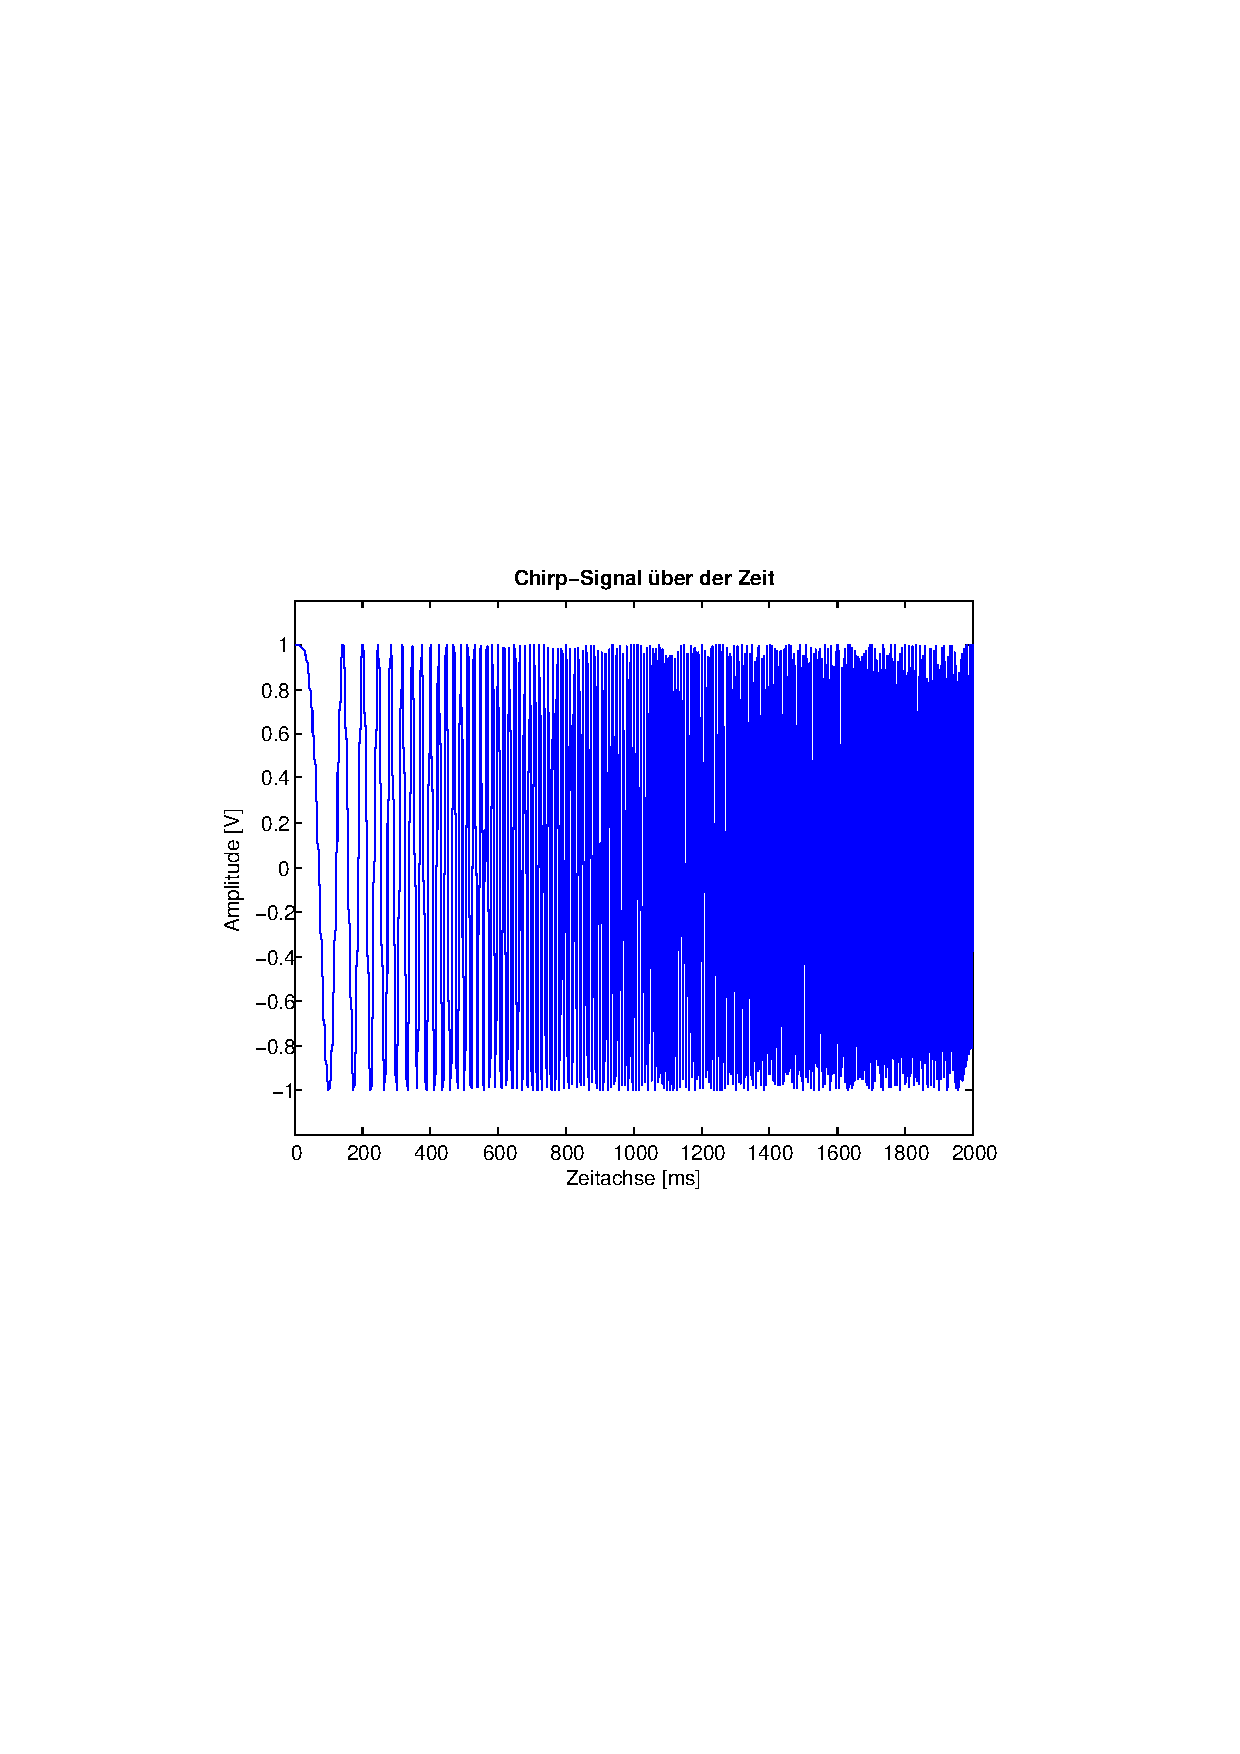
\includegraphics[scale=0.63, trim = 3cm 9cm 3cm
                            9cm, clip]{./Bilder/bsp_chirp}
                            %FIXME [width=640px,
                             %height=474px]
                            \caption{erzeugtes Chirp-Signal über der Zeit}
                        \end{figure}
    
                    \end{minipage}
                    \begin{minipage}{0.6\textwidth}
    
                        \begin{figure}[H]
                            \label{fig:}
                            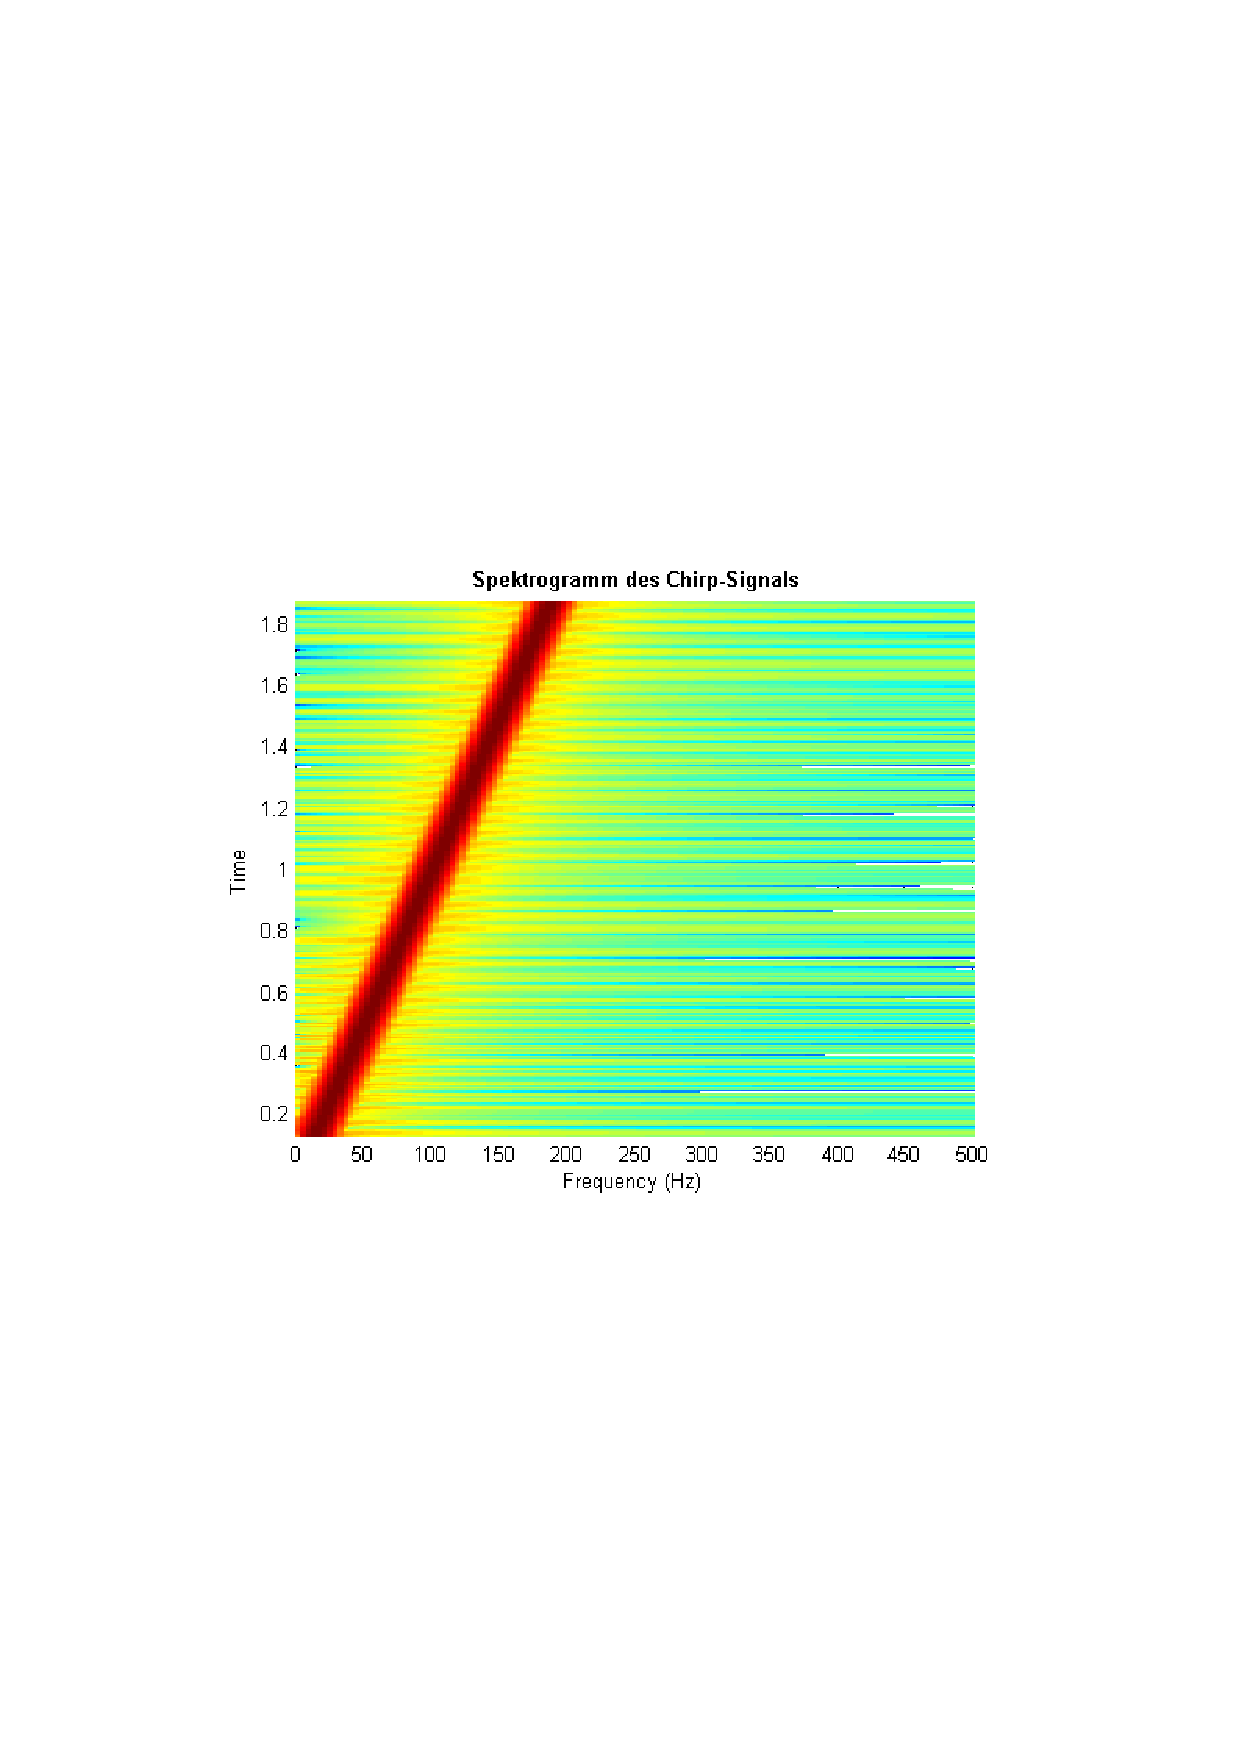
\includegraphics[scale=0.63, trim = 3cm 9cm 3cm
                            9cm,
                            clip]{./Bilder/bsp_chirp_spectrogram}
                            %FIXME [width=640px,
                             %height=474px]
                            \caption{Spektrogramm des erzeugten Chirp-Signals}
                        \end{figure}
                    \vspace{-1.5em}
    
                    \end{minipage}
    
                \end{tabular}
                \end{center}
                
                \vspace{1.5em}
        
        Man sieht einen Sinusverlauf, dessen Frequenz mit der Zeit immer größer
        wird. Wir vermuten einen linearen Abstieg der Frequenz. Im Spektrogramm
        kann man deutlich sehen, dass nach einer Sekunde die Frequenz den
        erwünschten Wert von $100 Hz$ annimmt.\\
        
        Weiterhin kann man die Auswirkung der Eingabevariablen des
        Spektrogrammaufrufs auf das entstehende Spektrogramm untersuchen. Hier
        sind zwei Beispiele, in denen einmal die Überlappungsfläche zwischen
        zwei Segmenten verkleinert wird und einmal die verwendete Fenstergröße
        vergrößert wird.
        
        
            \begin{center}
                \begin{tabular}{ll}
    
                \hspace{-12em}
                    \begin{minipage}{0.6\textwidth}
    
                        \begin{figure}[H]
                            \label{fig:}
                            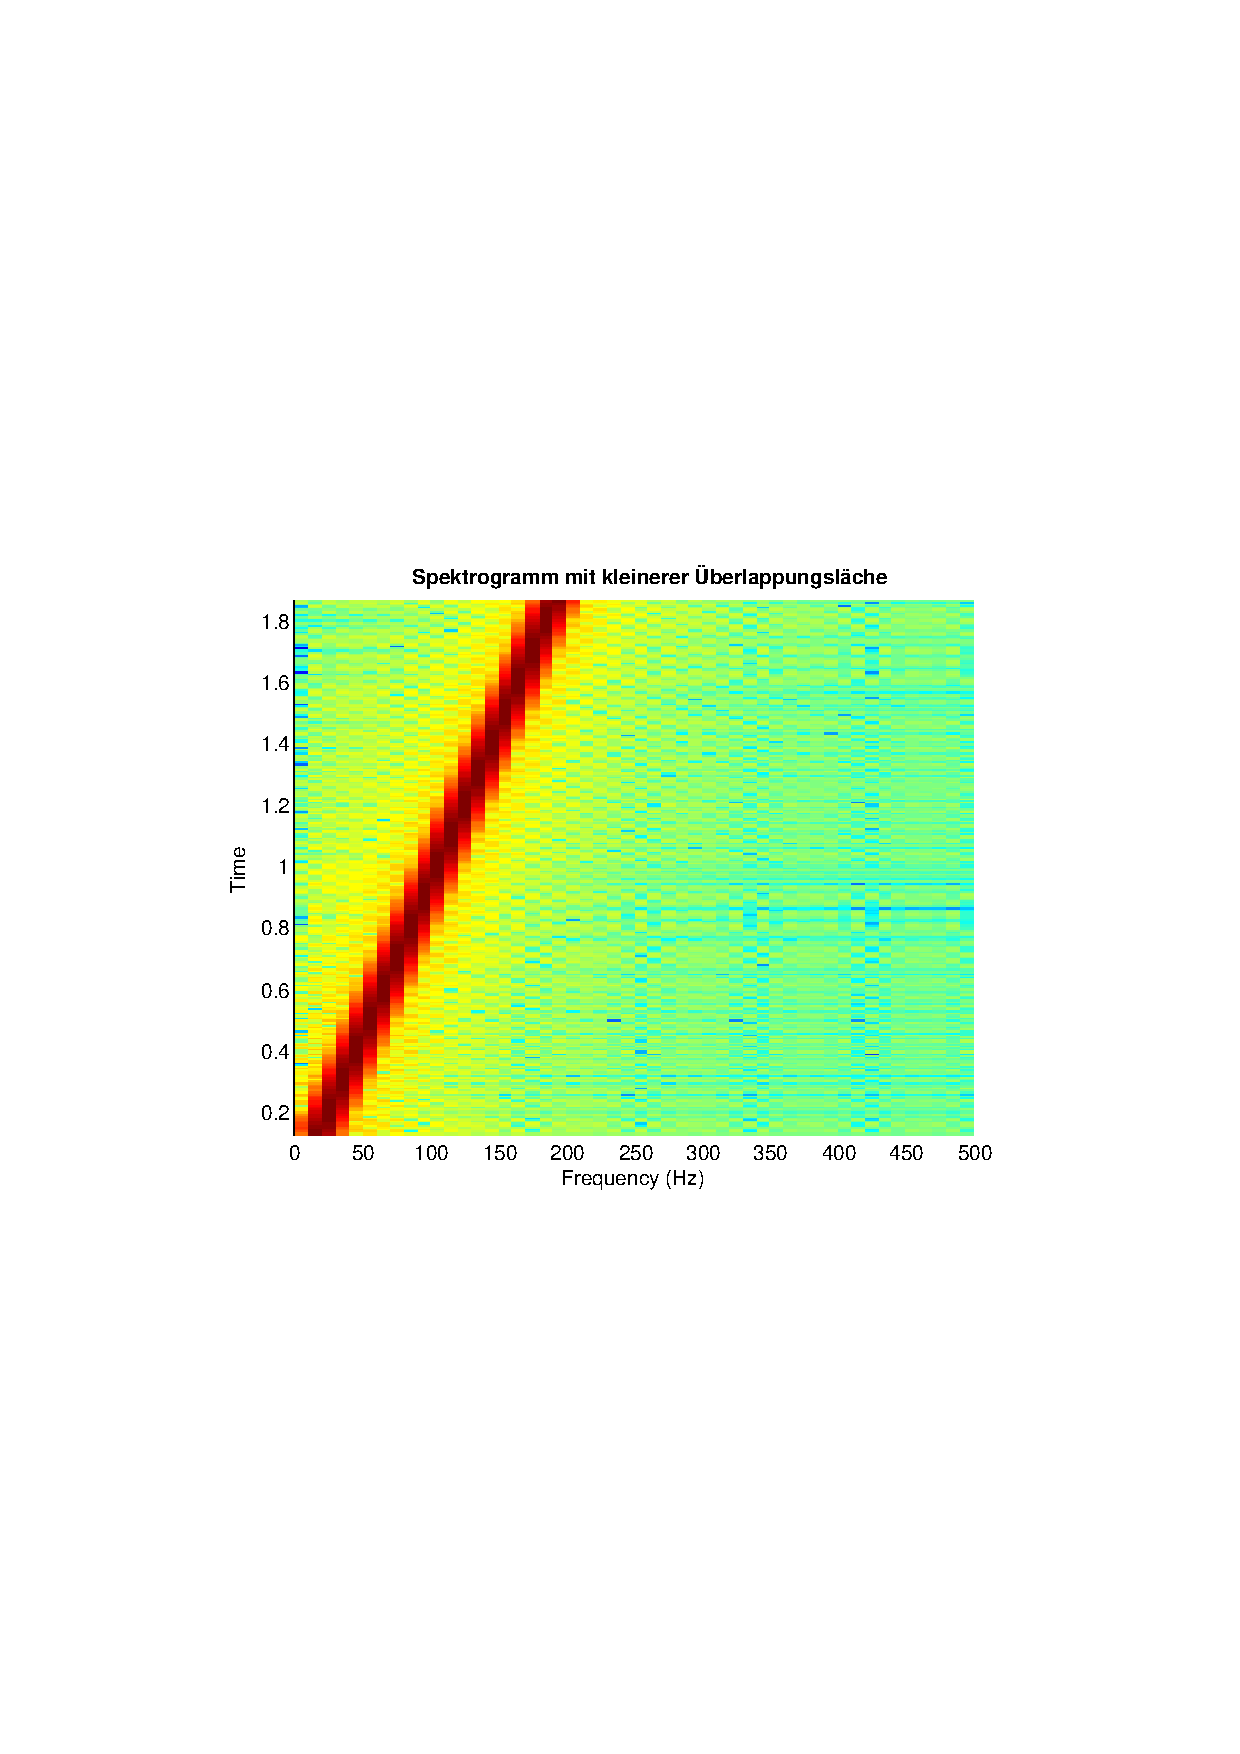
\includegraphics[scale=0.63, trim = 3cm 9cm 3cm
                            9cm,
                            clip]{./Bilder/bsp_chirp_spectrogram_kleineUeberlappung}
                            %FIXME [width=640px,
                             %height=474px]
                            \caption{Überlappung zwischen den Segmenten im
                            Spektrogram wird kleiner gewählt}
                        \end{figure}
    
                    \end{minipage}
                    \begin{minipage}{0.6\textwidth}
    
                        \begin{figure}[H]
                            \label{fig:}
                            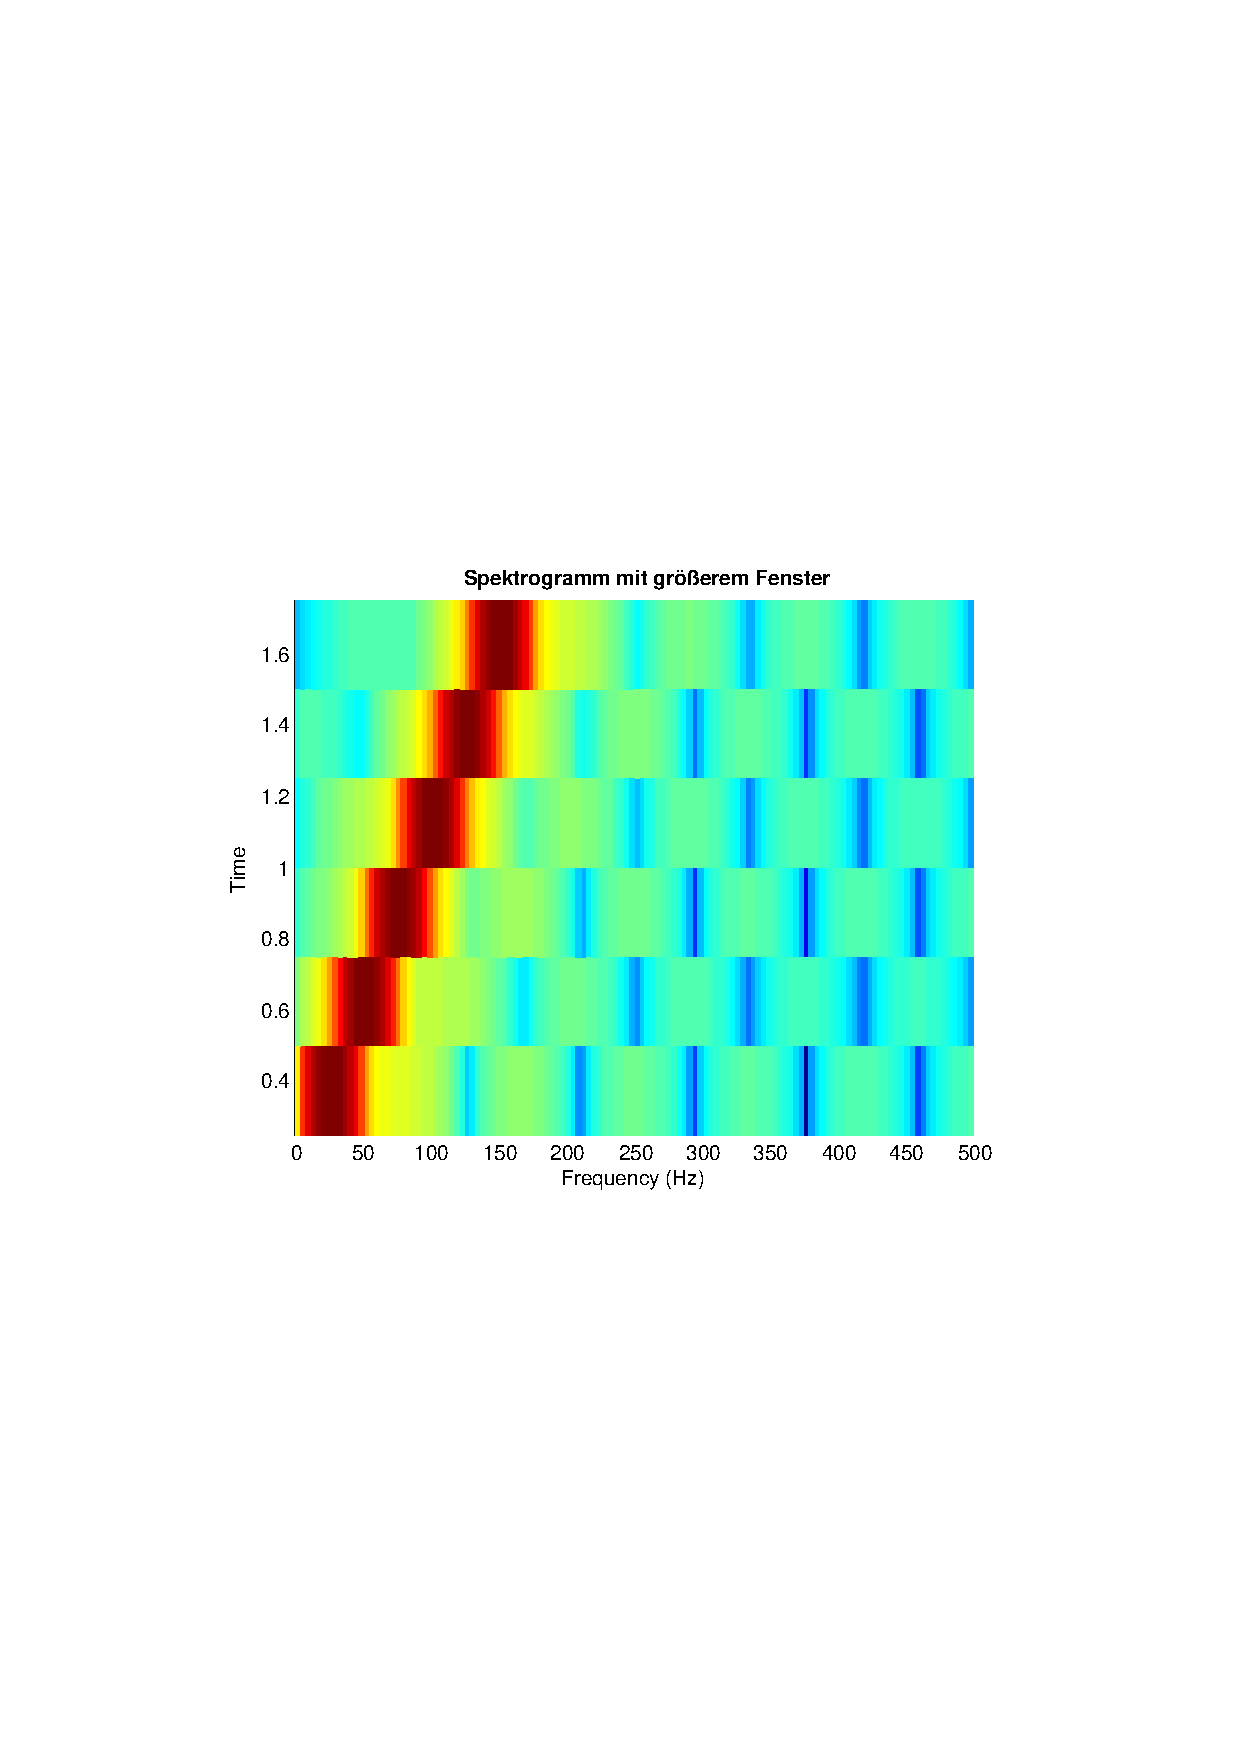
\includegraphics[scale=0.63, trim = 3cm 9cm 3cm
                            9cm,
                            clip]{./Bilder/bsp_chirp_spectrogram_grossesFenster}
                            %FIXME [width=640px,
                             %height=474px]
                            \caption{verwendete Fensterfolge wird größer
                            gewählt}
                        \end{figure}
                    \vspace{-1.5em}
    
                    \end{minipage}
    
                \end{tabular}
                \end{center}
                
                \vspace{1.5em}
        
        Innerhalb des gewählten Fensters, kann das verwendete Signal als
        stationär angenommen werden. Wird das Beobachtungsfenster kürzer, nimmt
        auch die Frequenzauflösung ab. Wird das Fenster zu groß, kann wiederum
        das Signal innerhalb des Fensters nicht mehr als stationär angenommen
        werden. Die Verschlechterung und Ungenauigkeiten im Spektrogramm kann
        man in den Plots oben gut erkennen.
        
        \end{quote}%ende Chirp-Signal erzeugen
	    
	    \subsubsection{Matlab-Funktion: Frequenzverlau über der Zeit}
	    \begin{quote}
	    
	    Als nächstes sollte eine Matlab-Funktion erstellt werden, die im
	    Zeitbereichdie momentane Frequenz ermittelt. Dieser berechnete
	    Frequenzverlauf über der Zeit sollte geplottet und mit dem erwarteten
	    Verlauf verglichen werden. In die erstellte Funktion kann in den Codes am
	    Ende des Protokolls eingesehen werden. Der entstandene Plot ist hier zu
	    sehen:
	    
	    \begin{figure}[H]
                    \centering
                        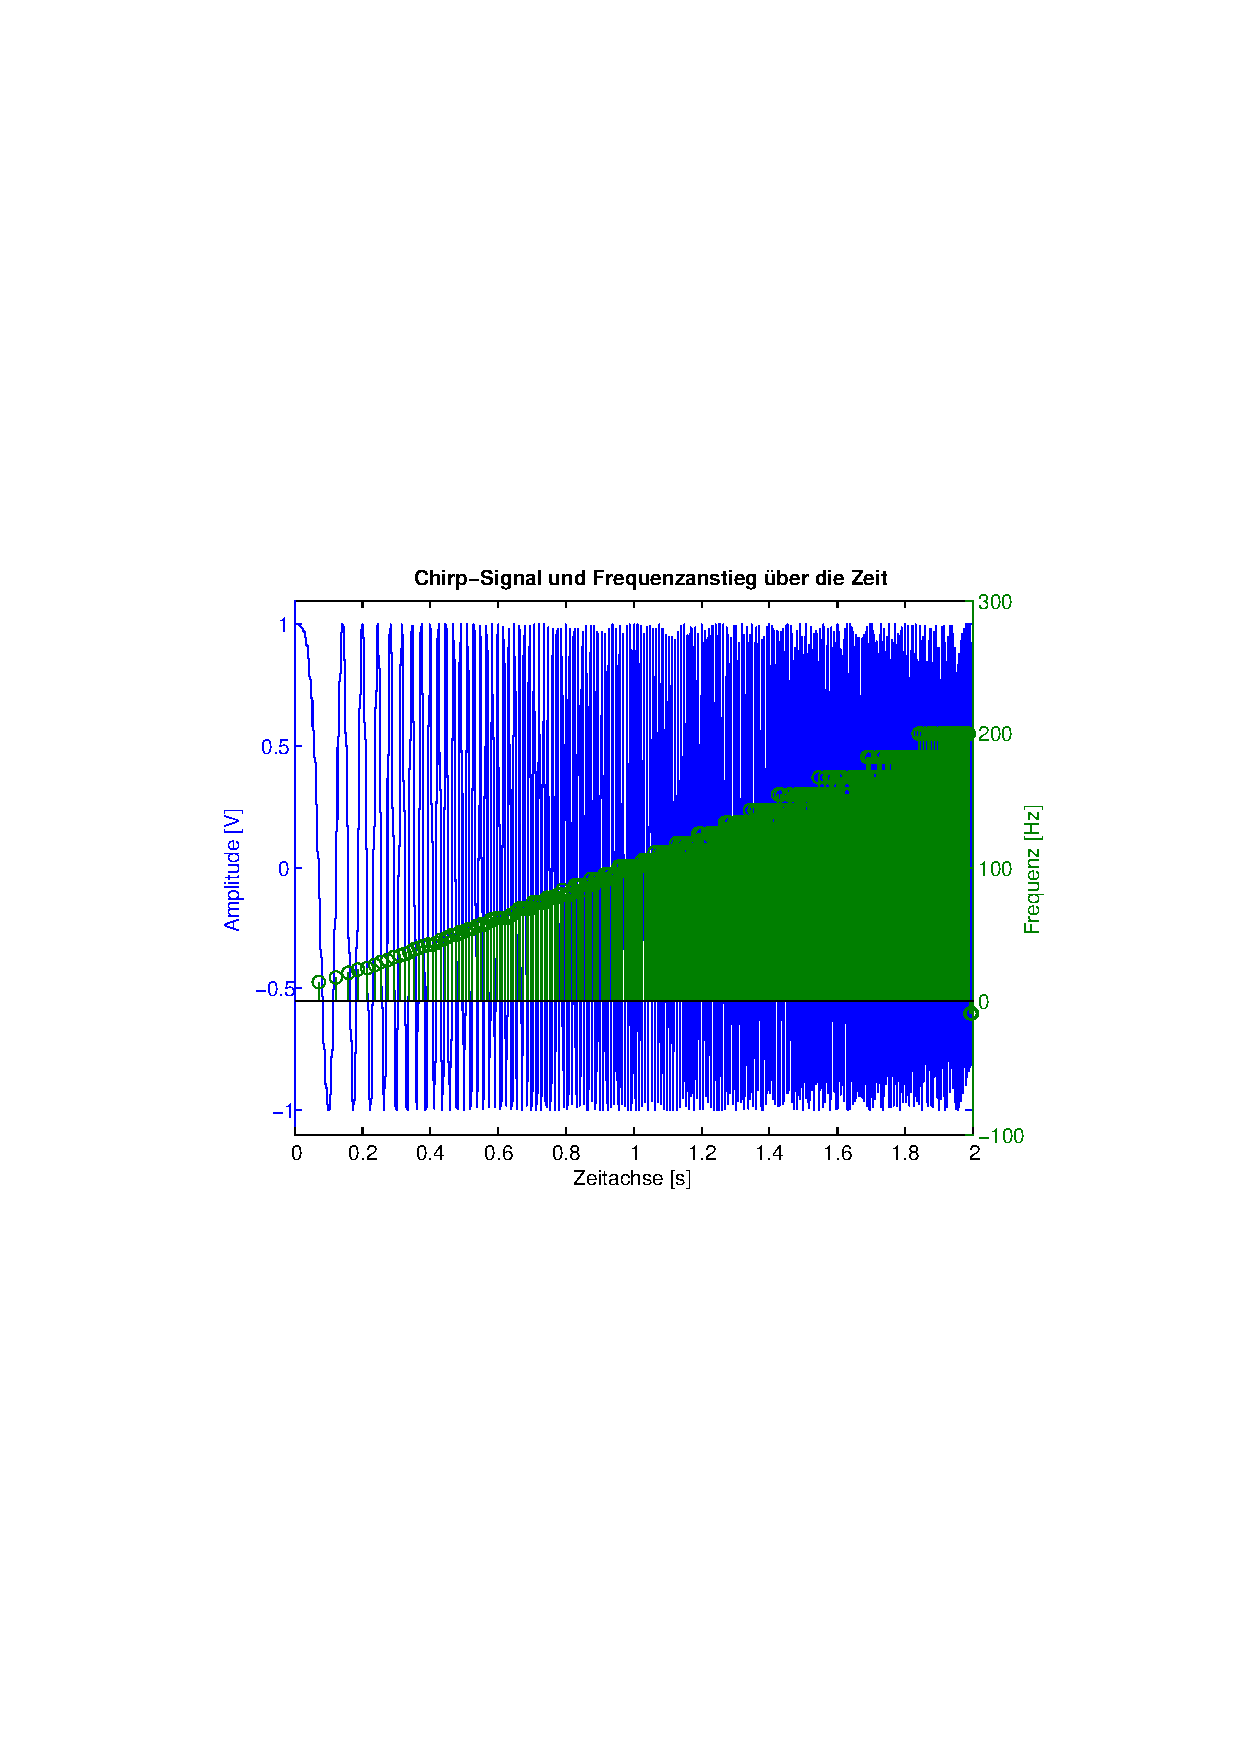
\includegraphics[scale=0.7, trim = 1cm 9cm 1.5cm 8cm,
                        clip]{./Bilder/chirpsignal_vs_frequenzanstieg}
                            \caption{Chirp-Signal und der dazugehörige
                            Frequenzanstieg, berechnet aus dem Zeitsignal}
                            \label{fig:./Bilder/chirpsignal_vs_frequenzanstieg}
                    \end{figure}
	    \end{quote}
	    
	    Da beim Erstellen des Chirpsignals ein linearer Ansteig der Frequenz
	    vorausgesetzt war, wurde auch ein linearer Frequenzverlauf erwartet. Das
	    Ergebnis bestätigt die Erwartung.
	    
	    \end{quote}% ende Matlab-Funktion: Frequenzverlauf über der Zeit
	    
	    \subsubsection{Matlab-Funktion: Frequenzverlauf anhand Spektrogram}
	    \begin{quote}
	    
	    Nun sollte der gleiche Frequenzverlauf anhand des Spektrogramms ermittelt
	    werden. Dafür implementierten wir eine weitere Matlab-Funktion, welche in
	    den Codes zu sehen ist. Das erwartete Ergebnis war wieder ein positiver
	    linearer Anstieg.
	    
	    \begin{figure}[H]
                    \centering
                        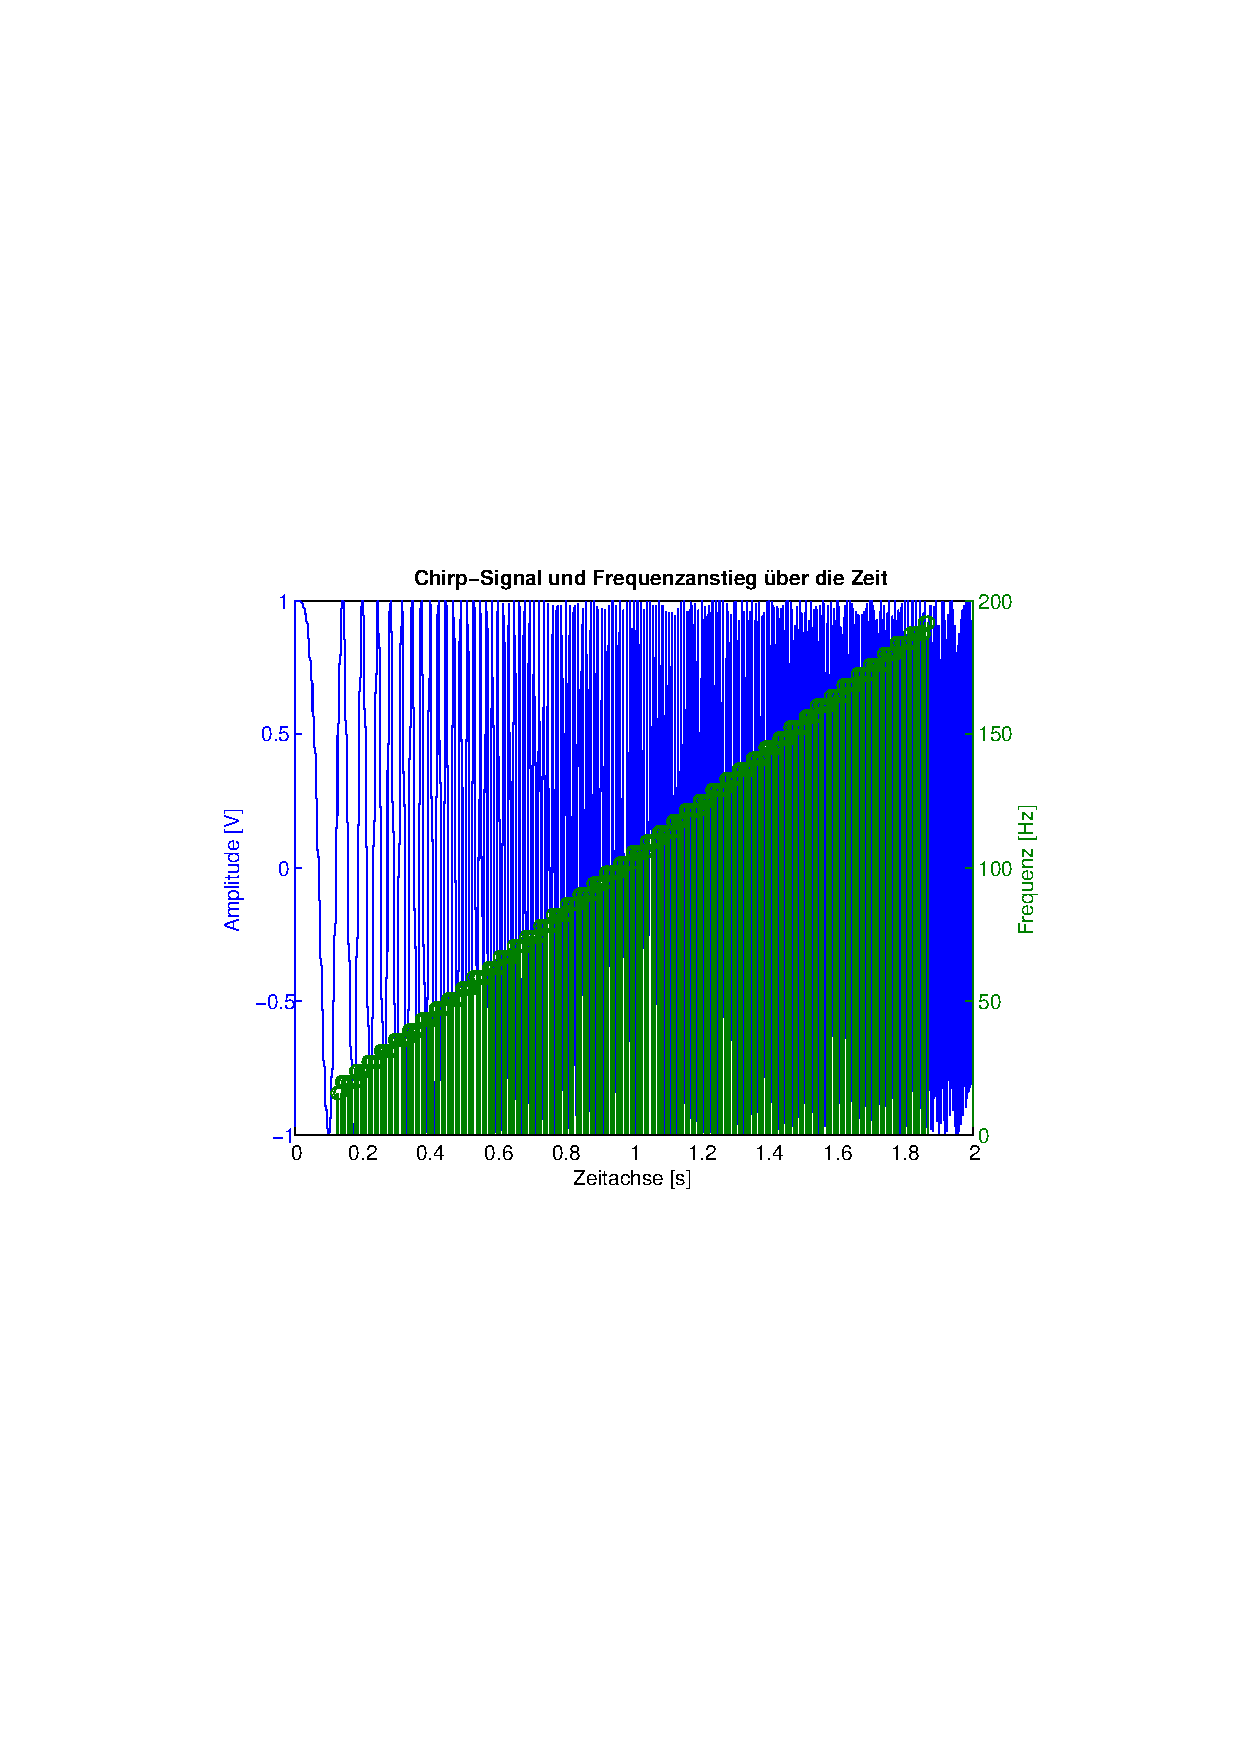
\includegraphics[scale=0.7, trim = 1cm 9cm 1.5cm 8cm,
                        clip]{./Bilder/chirpsignal_vs_frequenzanstieg_spectrogram}
                        \caption{Chirp-Signal und der dazugehörige
                            Frequenzanstieg, berechnet aus dem Spektrogramm}
                            \label{fig:./Bilder/chirpsignal_vs_frequenzanstieg_spectrogram}
                    \end{figure} 
	        
	    \end{quote}% ende Matlab-Funktion: Frequenzverlauf anhand Spektrogram
         
	    \subsubsection{Drehzahl-Berechnung anhand Amplitudenspektrum des
	    Motorstroms}
	    \begin{quote}
	    
	    Zuletzt wurde die Drehzahl des verwendeten Motors berechnet. Dafür wurden
	    uns drei Messreihen mit jeweils Strom- und Tachomesswerten vorgegeben.
	    Zunächst sollten die Amplitudenspektren der Motorströme erstellt werden,
	    welche uns durch die DFT der Stromwerte gelang. Die erhöhten Amplitudenwerte entsprachen
	    dabei den einfachen Vielfachen der Drehfrequenz des Motors mit der
	    jeweiligen Versorgungsspannung. Die deutlich herausstehenden Peaks dagegen
	    traten nur bei dem 18- oder 36-fachen Vielfachen der Drehfrequenz auf.
	    Dieses Wissen nutzen wir, indem wir anhand eines Matlabalgorithmuses den
	    höhsten Peak mit Index ausgaben lassen (die höchsten Peaks waren stets
	    jene, die am nächsten zu der null standen), um daraus eine Frequenz zu
	    bestimmen und durch 18 zu teilen. So berechneten wir die drei geforderten
	    Drehfrequenzen. Der Algorithmus steht in den Codes, die drei
	    Amplitudenspektren sehen folgendermaßen aus:
	    
	     \begin{center}
                \begin{tabular}{ll}
    
                \hspace{-12em}
                    \begin{minipage}{0.6\textwidth}
    
                        \begin{figure}[H]
                            \label{fig:}
                            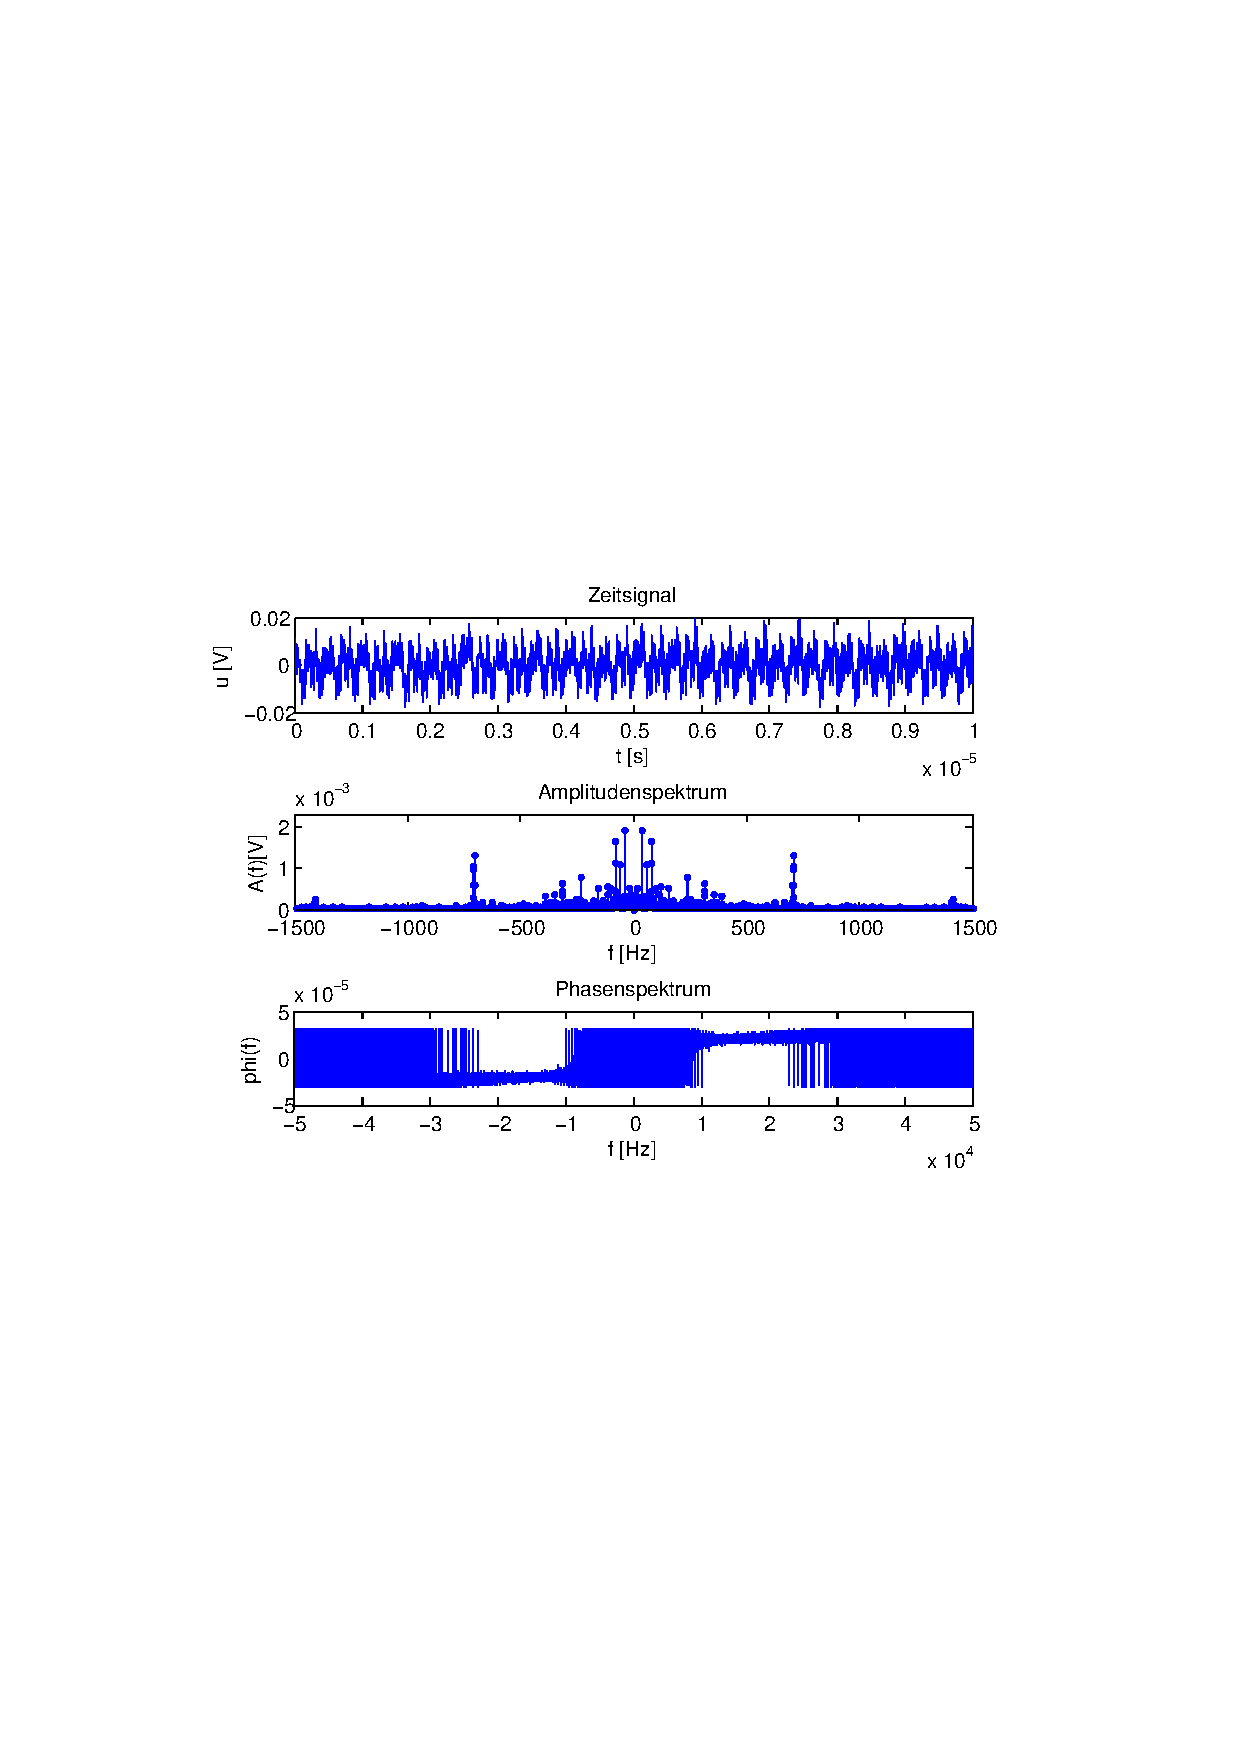
\includegraphics[scale=0.63, trim = 3cm 9cm 3cm
                            8.5cm, clip]{./Bilder/ampl_spektrum_messung1}
                            %FIXME [width=640px,
                             %height=474px]
                            \caption{Spektrum des Motorstroms bei 10V}
                        \end{figure}
    
                    \end{minipage}
                    \begin{minipage}{0.6\textwidth}
    
                        \begin{figure}[H]
                            \label{fig:}
                            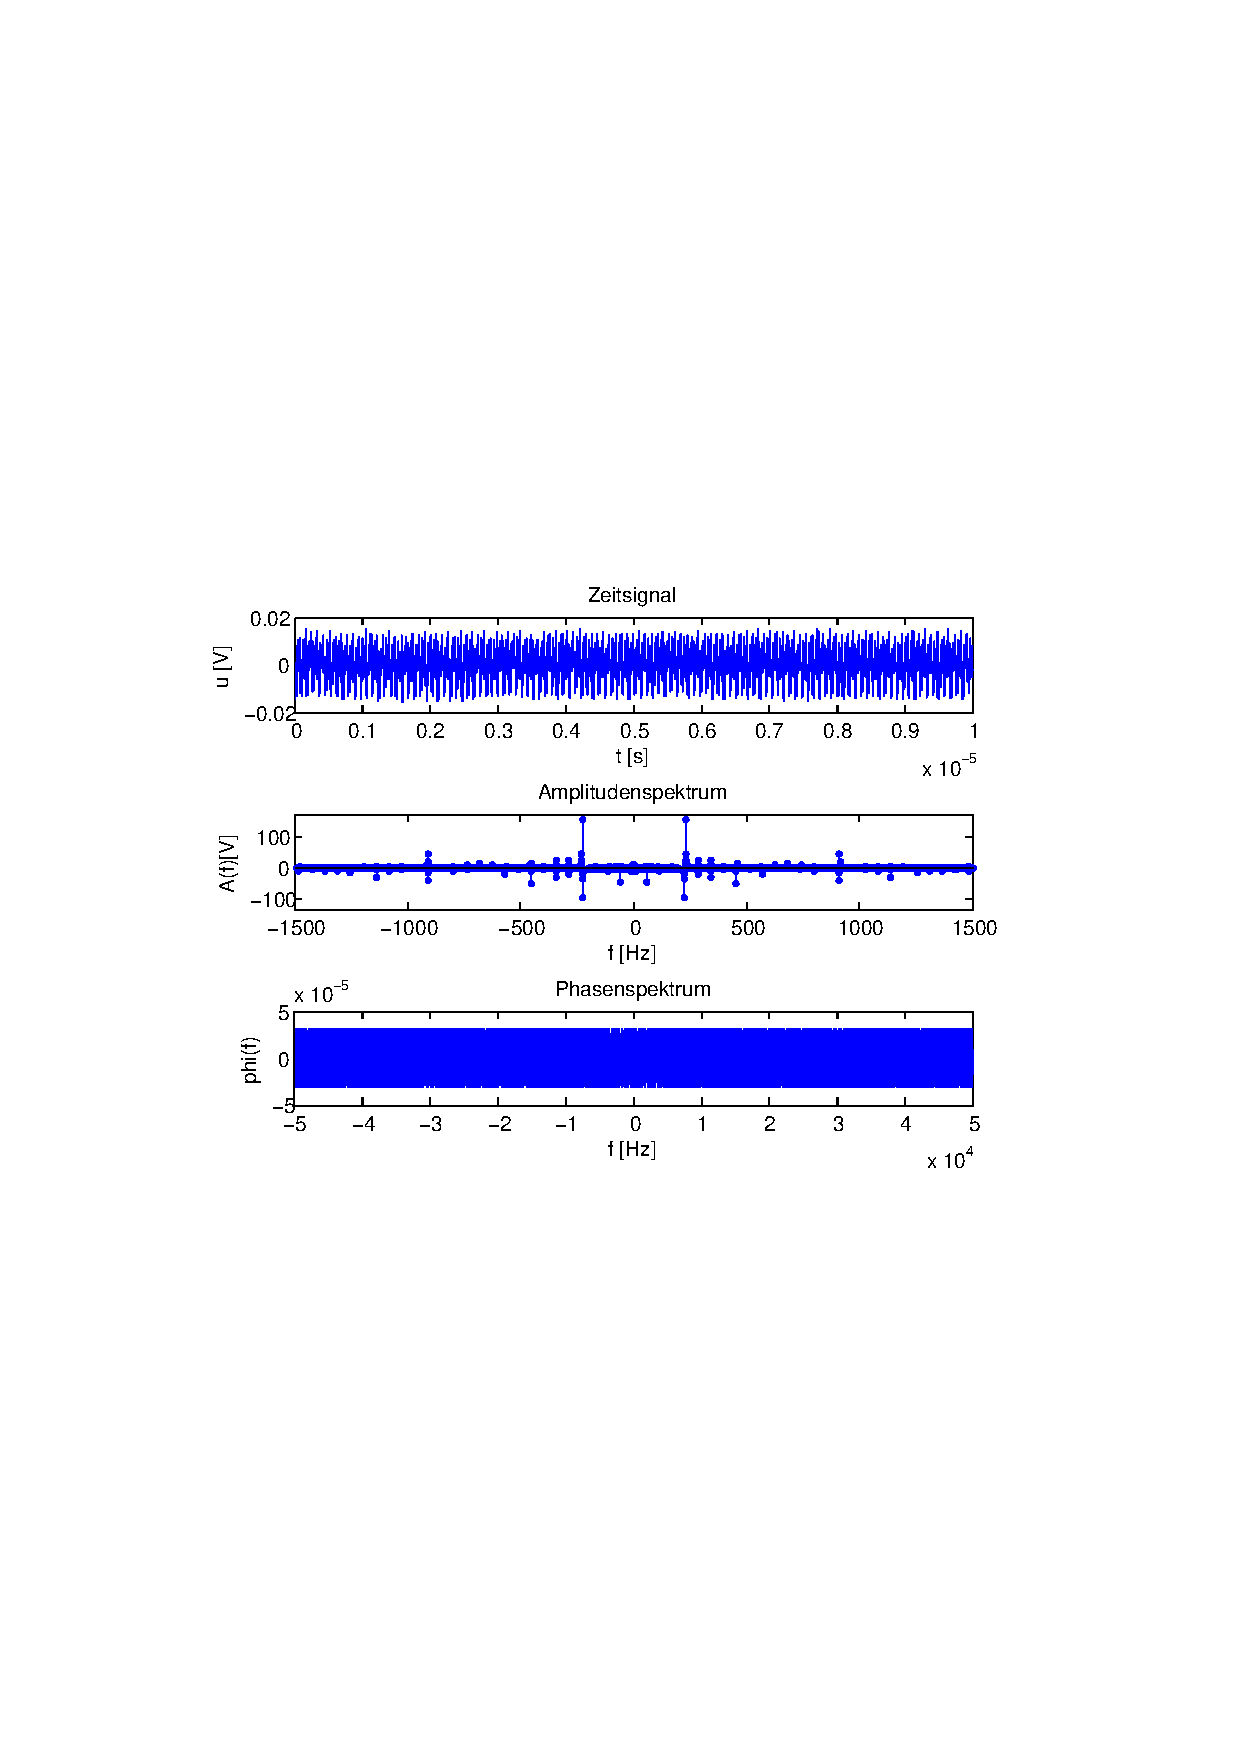
\includegraphics[scale=0.63, trim = 3cm 9cm 3cm
                            8.5cm,
                            clip]{./Bilder/ampl_spektrum_messung2}
                            %FIXME [width=640px,
                             %height=474px]
                            \caption{Spektrum des Motorstroms bei 20V}
                        \end{figure}
                    \vspace{-1.5em}
    
                    \end{minipage}
    
                \end{tabular}
                \end{center}
	           
	           
	           \begin{figure}[H]
                    \centering
                        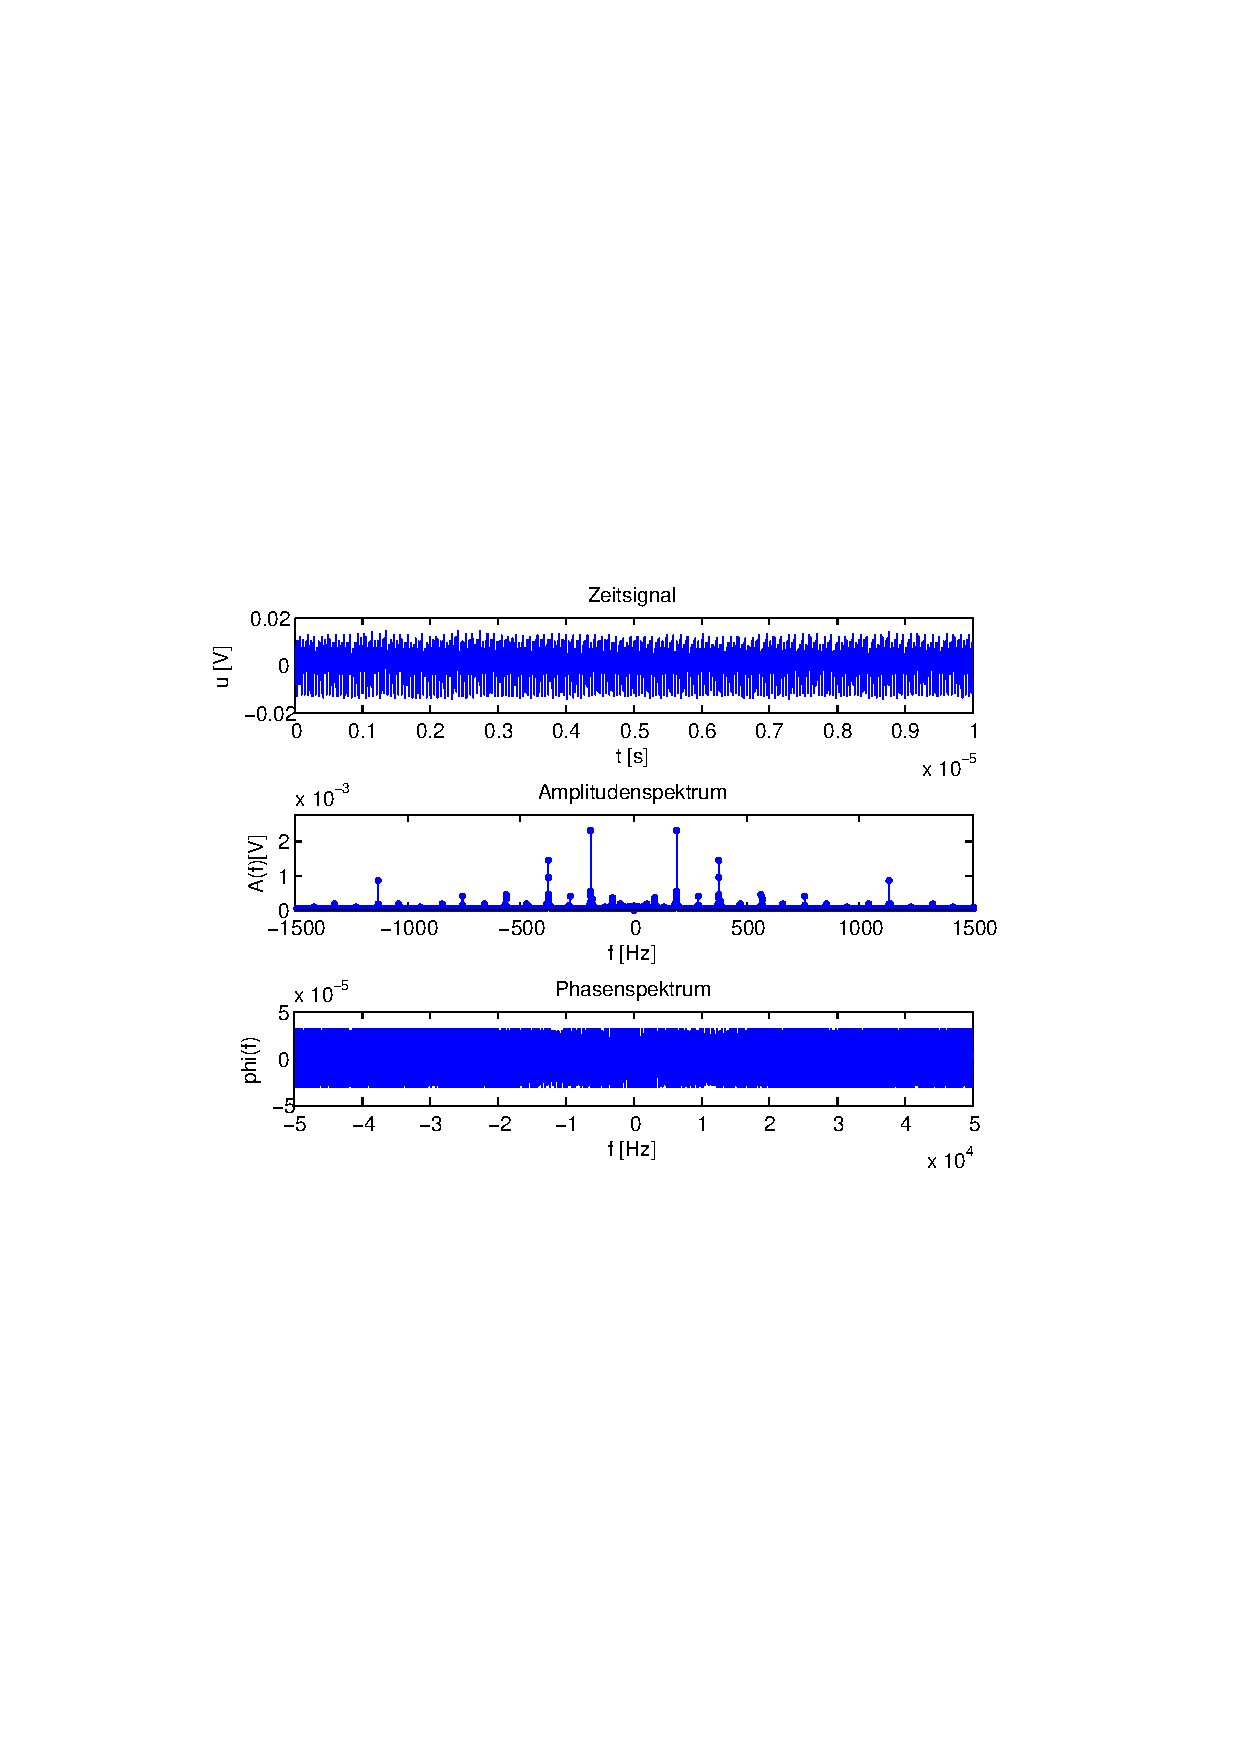
\includegraphics[scale=0.63, trim = 1cm 9cm 1.5cm 8cm,
                        clip]{./Bilder/ampl_spektrum_messung3}
                        \caption{Spektrum des Motorstroms bei 30V}
               \end{figure}
	    
	    Die berechneten Drehfrequenzen betragen für die erste Messung ($10V$) =
	    $2.1389 Hz$, für die zweite Messung ($20V$) = $6.3056 Hz$ und für die
	    dritte Messung ($30V$) = $10.4723 Hz$.\\
	    
	    \TODO{Hier sind die Werte falsch, weil wir die falschen Paeks rausgesucht
	    haben, Fehler muss noch korrigiert werden}
	    
	    Außerdem wurden die Drehfrequenzen auch aus den jeweiligen Tachosignalen
	    bestimmt. Dafür wurde genauso vogegangen wie bei den Motorströmen. Die
	    Spektren sind hier:
	       
        \begin{center}
                \begin{tabular}{ll}
    
                \hspace{-12em}
                    \begin{minipage}{0.6\textwidth}
    
                        \begin{figure}[H]
                            \label{fig:}
                            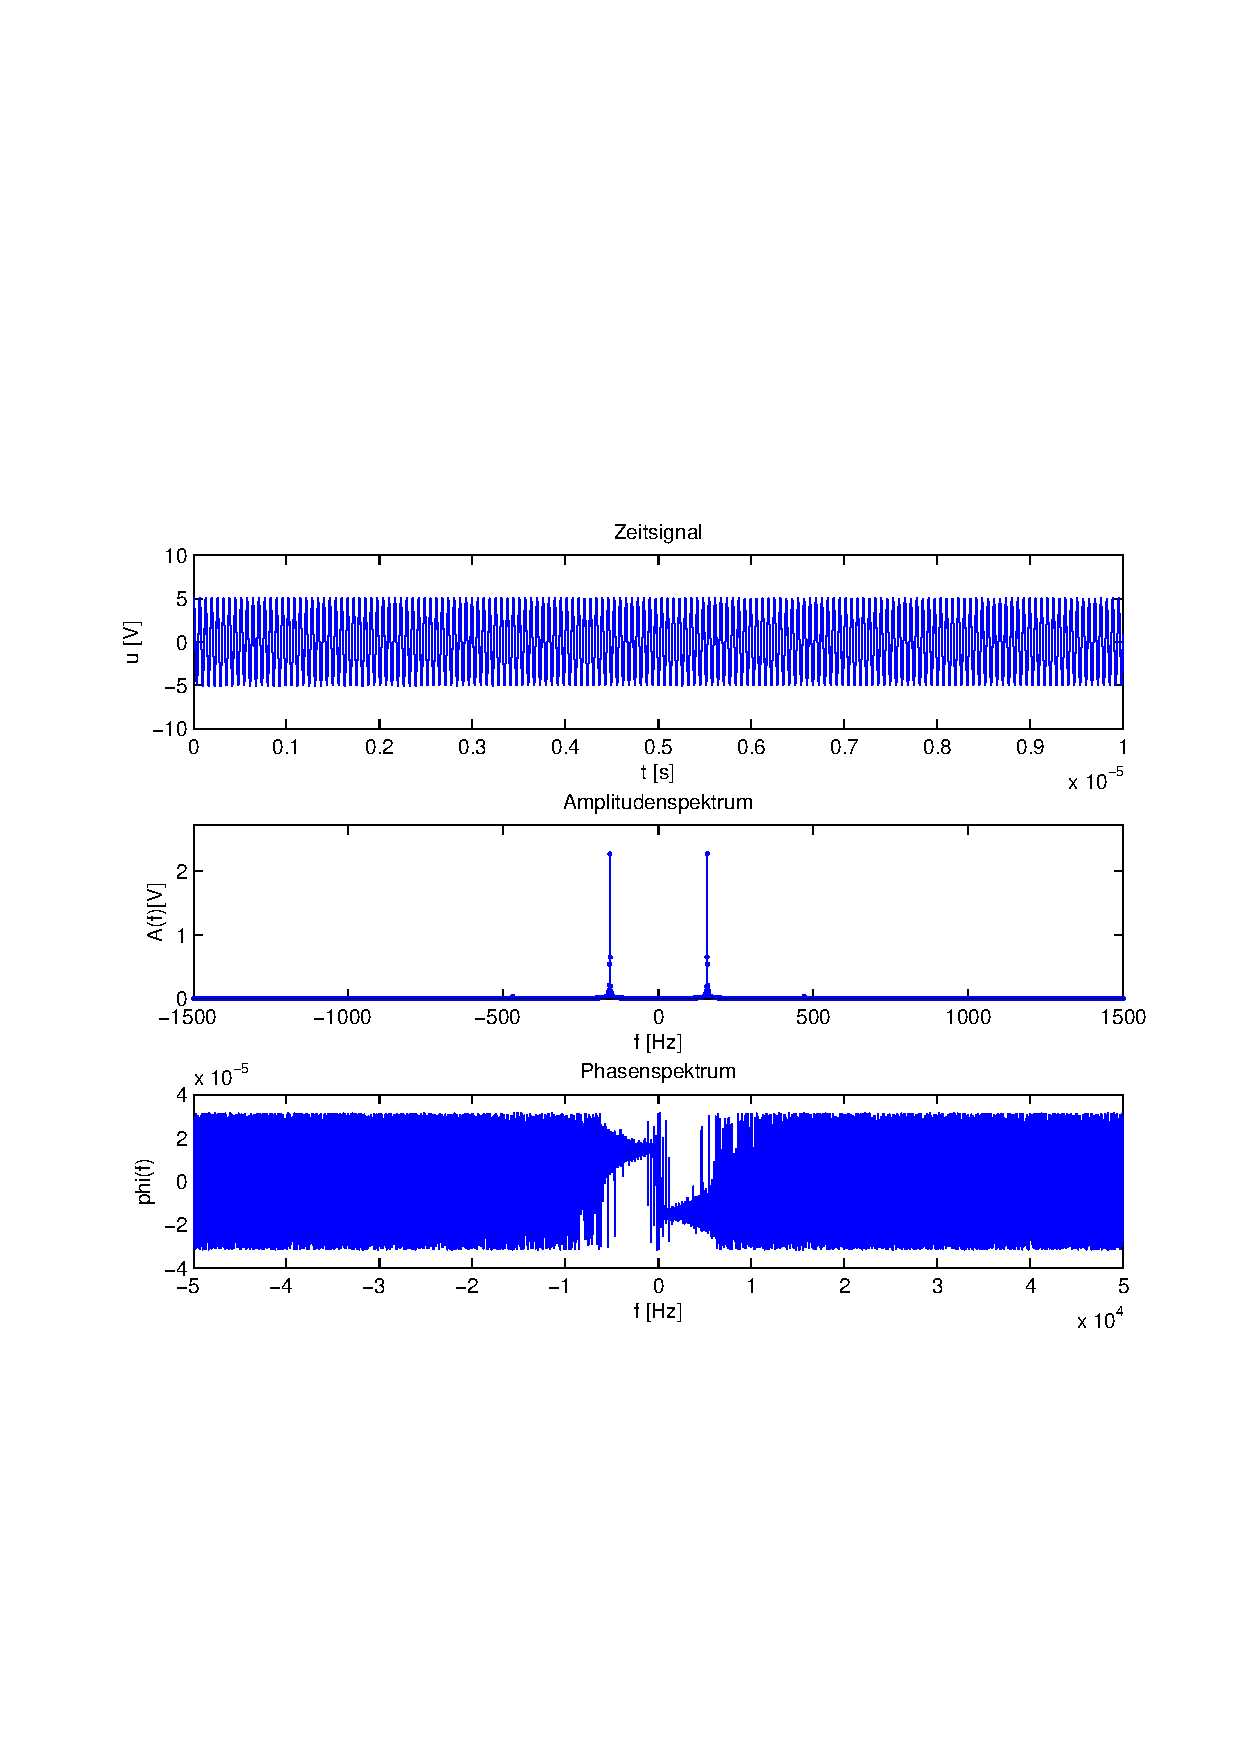
\includegraphics[scale=0.45, trim = 0.8cm 7cm 3cm
                            8.5cm, clip]{./Bilder/ampl_spektrum_messung1_tacho}
                            %FIXME [width=640px,
                             %height=474px]
                            \caption{Spektrum des Tachosignals bei 10V}
                        \end{figure}
    
                    \end{minipage}
                    \begin{minipage}{0.6\textwidth}
    
                        \begin{figure}[H]
                            \label{fig:}
                            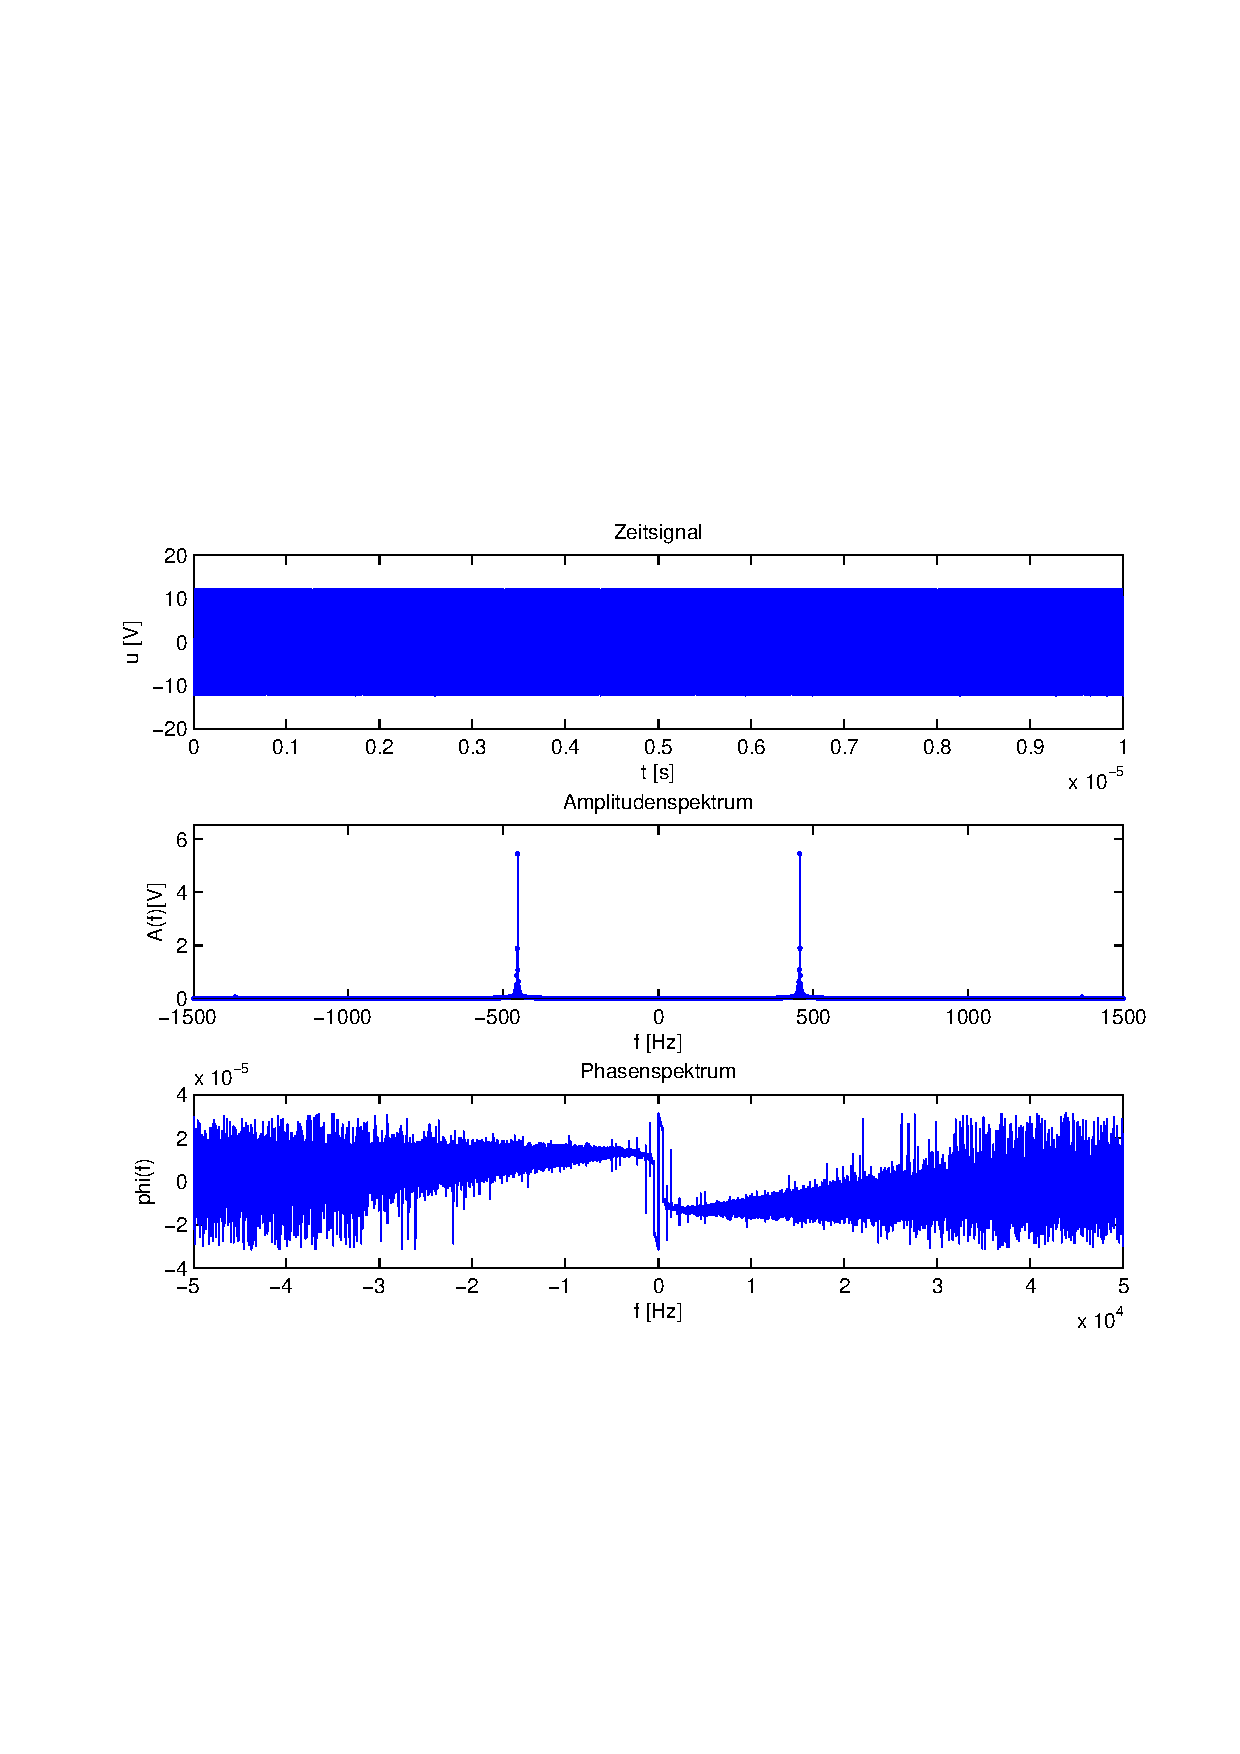
\includegraphics[scale=0.45, trim = 0.8cm 7cm 3cm
                            8.5cm,
                            clip]{./Bilder/ampl_spektrum_messung2_tacho}
                            %FIXME [width=640px,
                             %height=474px]
                            \caption{Spektrum des Tachosignals bei 20V}
                        \end{figure}
                    \vspace{-1.5em}
    
                    \end{minipage}
    
                \end{tabular}
                \end{center}
               
               
               \begin{figure}[H]
                    \centering
                        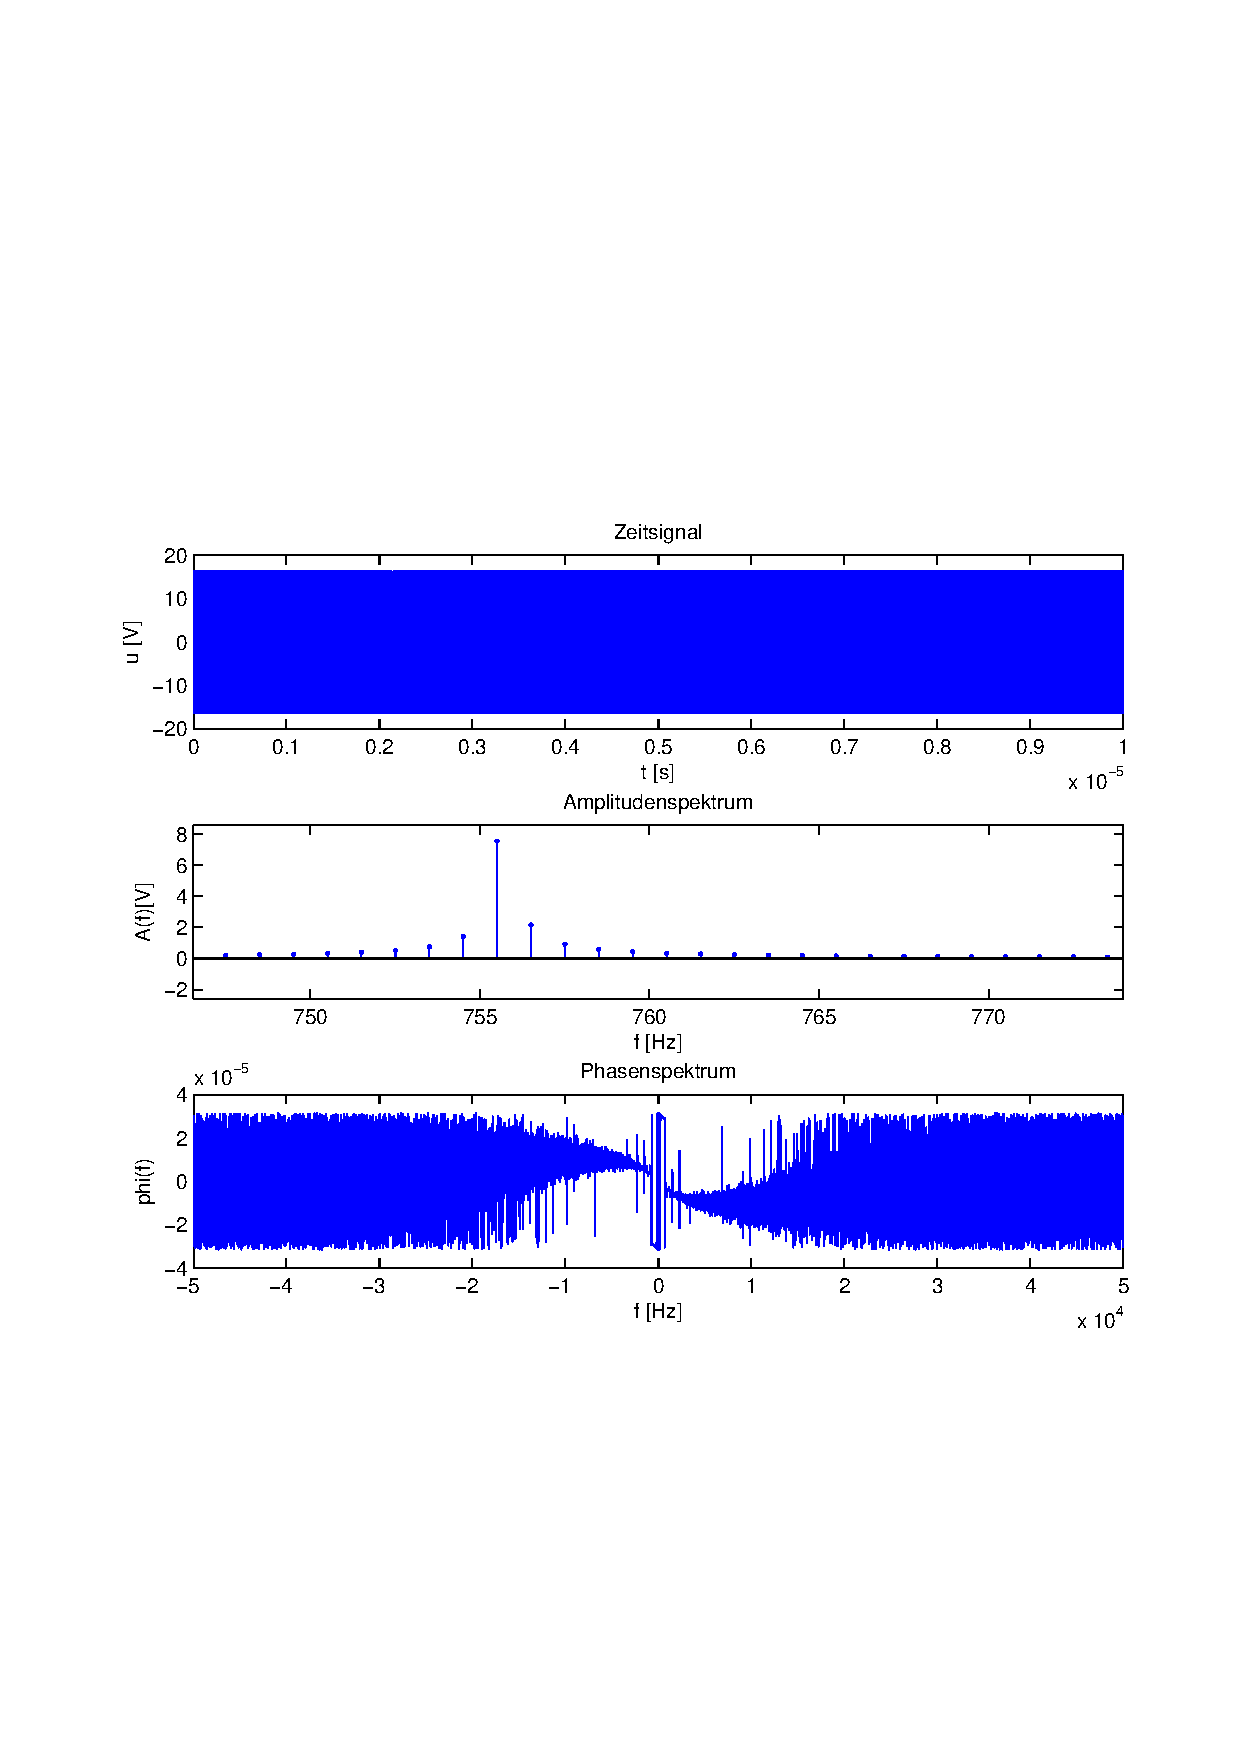
\includegraphics[scale=0.45, trim = 0.8cm 7cm 1.5cm 8cm,
                        clip]{./Bilder/ampl_spektrum_messung3_tacho}
                        \caption{Spektrum des Tachosignals bei 30V}
               \end{figure}
               
        Die anhand der Tachosignale berechneten Drehfrequenzen betragen für die
        erste Messung ($10V$) = $19.5627 Hz$, für die zweite Messung ($20V$) =
        $56.8131 Hz$ und für die dritte Messung ($30V$) = $94.3134 Hz$.\\
	    Es fällt auf, dass die Drehzahlen, welche über die Ströme berechnet werden,
	    ca. 4mal kleiner sind als die Drehzahlen über die Tachowerte. Ein
	    konstanter Faktor von 4 kann angenommen werden.
	    
	    \end{quote}%ende Drehzahl-Berechnung anhand Amplitudenspektrum des
	    % Motorstroms
        
	    
	\end{quote}
	
    \subsection{Vorbereitungsaufgaben zu Termin 8}
    \begin{quote}
    
        \subsubsection{Zerlegung des Signals mittels Haar-Tranformation}
        \begin{quote}
        
        In der ersten Vorbereitungsaufgabe des 8.Praktikumstermins wird eine
        vorgegebene strom.m Datei verwendet, welche einen angechnittenen Sinus
        im Bereich $[0,8\pi]$ darstellt. Dieses Signal wird mit der Schnellen
        Haar-Transformation zerlegt. Außerdem wird die Approximation und die
        Details dür die Skalierungen $m = 1 \ldots 5$ berechnet werden, wofür
        die drei Funktionen haardec.m, haardeclevel.m und getAppDet.m
        implementiert werden. Diese stehen unter den Codes.
        
        \end{quote}%ende Zerlegung des Signals mittels Haar-Transformation
        
        
        \subsubsection{Darstellung der Approximationen}
        \begin{quote}
        
        Als nächstes werden die Approximationen und die Details des
        angeschnittenen Sinus-Signals dargestellt und das stationäre Spektrum
        sowie das Spektrogramm berechnet. Diese spektralen Darstellungen werden
        mit den Darstellungen mittels Wavelets verglichen. Am Ende soll
        ermittelt werden, welche Darstellung bestimmte Informationen über das
        verwendete Signal besser veranschaulicht.
        
        \TODO{entsprechende Ergebnisse einfügen}
        
        \end{quote}%ende Darstellung der Approximationen
        
        
        \subsubsection{Daubechies-Wavelets}
        \begin{quote}
        
        Nun wird das angeschnitte Sinus-Signal mit Hilfe von Daubechies-Wavelets
        zerlegt. Dazu verwenden wir die Matlab-Fuktionen wavedec, appcoef
        und detcoaf und variieren die Anzahl der verschwindenen
        Momente der Wavelets.
        
        \TODO{Ergebnisse einfügen}
        
        \end{quote}%ende Daubechies-Wavelets
        
        
        \subsubsection{Vergleich der Zerlegungen mittels
        Daubechies-Wavelets und Haar-Wavelets}
        \begin{quote}
        
        Zuletzt wird in der Vorbereitung des Praktikums die Zerlegungen mittels
        Daubechies-Wavelets mit den Zerlegungen mittels Haar-Wavelets
        verglichen. Die Unterschiede sind folgende:
        
        \TODO{Unterschiede untersuchen und einfügen}
       
        \end{quote}%ende Vergleich der Zerlegungen mittels
        %Daubechies-Wavelets und Haar-Wavelets
    
    \end{quote}%Ende Vorbereitungsaufgaben zu Termin 8

\end{quote}%Ende Vorbereitungsaufgaben

\section{Durchführungen}
\begin{quote}

		\subsection{Durchführung zu Termin 7}
		\begin{quote}
            
            
            
		\end{quote}%Ende der Durchführung von Termin 7

		\subsection{Durchführung zu Termin 8}
		\begin{quote}
            
            
            
		\end{quote}%Ende der Durchführungen von Termin 8

\end{quote}%Ende Durchführungen


%--------------------------------------------------------------------
%--------------------------------------------------------------------
\section{Auswertung}
\begin{quote}
	\subsection{Auswertung Termin 7}
    \begin{quote}

    \end{quote}  % Ende Subsection Auswertung Termin 7

    \subsection{Auswertung Termin 8}
    \begin{quote}


    \end{quote}  % Ende Subsection Auswertung Termin 8
\end{quote} %Ende section

%--------------------------------------------------------------------
%--------------------------------------------------------------------    


%--------------------------------------------------------------------
%--------------------------------------------------------------------
\section{Quellcodes}
\begin{quote}

	\subsection{Codes aus Termin 7}
	\begin{quote}
	    
	    \subsubsection{Frequenzverlauf über der Zeit}
	    \begin{quote}
	        \lstinputlisting[
	            caption={frequenz_imZeitbereich_ausSignal},
	            label=lst:Matlab]
	            {./Matlab/Termin7/frequenz_imZeitbereich_ausSignal.m}
	    \end{quote}

	    \subsubsection{Frequenzverlauf aus dem Spektrogram}
	    \begin{quote}
	        \lstinputlisting[
	            caption={frequenz_durch_Spektogramm},
	            label=lst:Matlab]
	            {./Matlab/Termin7/frequenz_durch_Spektogramm.m}
	    \end{quote}

        \subsubsection{Algorithmus zur Drehfrequenzberechnung}
        \begin{quote}
            \lstinputlisting[
                caption={Algorithmus zur Drehfrequenzberechnung},
                label=lst:Matlab]
                {./Matlab/Termin7/Vorbereitungsaufgabe4.m}
        \end{quote}
	    
	\end{quote}%ende Codes aus Termin7
	
	\subsection{Codes aus Termin 8}
	\begin{quote}
	
	   \subsubsection{Funktion haardec.m}
	   \begin{quote}
	   \lstinputlisting[
                caption={Funktion haardec.m},
                label=lst:Matlab]
                {./Matlab/Termin8/haardec.m}
	   \end{quote}
	   
	   \subsubsection{Funktion haardeclevel.m}
	   \begin{quote}
	   \lstinputlisting[
                caption={Funktion haardeclevel.m},
                label=lst:Matlab]
                {./Matlab/Termin8/haardeclevel.m}
	   \end{quote}
	   
	   \subsubsection{Funktion getAppDet.m}
	   \begin{quote}
	   \lstinputlisting[
                caption={Fuktion getAppDet.m},
                label=lst:Matlab]
                {./Matlab/Termin8/getAppDet.m}
	   \end{quote}
\end{quote}

%--------------------------------------------------------------------
%--------------------------------------------------------------------


%\begin{thebibliography}{999}
%\bibitem {Schaltungwandlerbox} Prof. Dr.-Ing. Gühmann, Clemens; Dipl.-Ing. Funk, Jürgen: MDVLaborGeraete_web, S.4

%Name, Vorname.; evtl. Name2, Vorname2.: Titel des Dokumentes
%oder Buches, Zeitschrift/Verlag/URL (Auflage, Erscheinungsort, -jahr), ggf. Seitenzahlen
%\bibitem {PasevalscheTheorem} \url{https://de.wikipedia.org/wiki/Parsevalsches_Theorem}, Zugriff
%23.05.2012
%\end{thebibliography}


\end{document}


